\section{Zielsetzung}
\label{sec:Zielsetzung}

Das Ziel des Experiments ist es, den Elastizitätsmodul mehrerer Metalle zu berechnen.
Dabei wird zur experimentellen Messung die Methode der Biegung gewählt, da diese am einfachsten durchzuführen ist.

\section{Theorie}
\label{sec:Theorie}

Ein Körper kann zu einem gewissen Maß unter Krafteinwirkung reversibel
verformt werden. Dieser Effekt wird Elastizität genannt. Im Folgenden soll nun
eine materialabhängige Konstante, der Elastizitätsmodul E, bestimmt werden
um eine relative Auslenkung $\increment L/L$ durch die senkrecht zur Oberfläche
wirkende Normalspannung $\sigma$ ausdrücken zu können. Diese Relation wird
Hooksches Gesetz genannt.

\begin{equation}
  \sigma = \symup{E}\frac{\increment L}{L}
  \label{eqn:hook}
\end{equation}

Wie bereits erwähnt soll eben dieser Elastizitätsmodul durch die
Durchbiegung $D(x)$ eines schmalen Metallstabes der Länge L, welcher an
einem Ende eingespannt und am anderen mit einem Gewicht versehen
beziehungsweise an beiden Seiten eingespannt und in der Mitte
mit einem Gewicht versehen ist, berechnet werden.
\begin{figure}
  \centering
  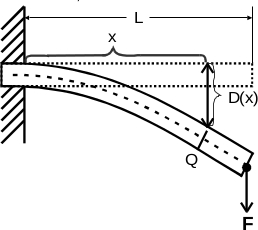
\includegraphics[width=0.3\textwidth]{content/images/Abbildung1.jpg}
  \caption{Durchbiegung eines elastischen Stabes.}
  \label{fig:abb1}
\end{figure}
Es ist wichtig zu beachten, dass die relative Längenänderung im Querschnitt
Q im Falle einer Biegung nicht konstant ist. Die Durchbiegung ist nun also
vom Ort abhängig.

\begin{equation}
  D \to D(x)
\end{equation}
In der Mitte des Stabes befindet sich eine Fläche an welcher
keine Spannung auftritt, die sogenannte neutrale Faser. Überhalb dieser
bildet sich eine Zugspannung (Streckung des Materials), untehalb eine Druckspannung
(Stauchung des Materials), welche zusammen durch Intergration über Q ein inneres Drehmoment $M_\sigma$ bilden.
Dieses muss mit dem äußeren Drehmoment $M_\symup{F}$ ins Gleichgewicht kommen.
\begin{equation}
  \begin{split}
    \label{eqn:dreh}
    M_\sigma &= \int_\symup{Q} y \sigma(y) \symup{d} \, q\\
    =M_\symup{F} &= F(L-x)
  \end{split}
\end{equation}
Durch die infnitesimale Betrachtung von \eqref{eqn:hook} und \eqref{eqn:dreh} ergibt
sich für die Durchbiegung $D(x)$ des einseitig eingespannten Stabes:
\begin{align}
  D(x) &= \frac{F}{2E\symbf{I}}\left(Lx^2-\frac{x^3}{3}\right)\\
\end{align}
Für den Kreis des Radius $R$ ergibt sich für das Flächenträgheitsmoment:
\begin{equation}
  \symbf{I}=I_\symup{x}=I_\symup{y}=\frac{\pi}{4}R^4
  \label{eqn:Ikreis}
\end{equation}
Für das Quadrat der Seitenlänge $a$ ergibt sich für das Flächenträgheitsmoment:
\begin{equation}
  \symbf{I}=I_\symup{x}=I_\symup{y}=\frac{a^4}{12}
  \label{eqn:Iquadrat}
\end{equation}
\begin{align}
\iff E &= \frac{F}{2\symbf{I}D(x)}\left(Lx^2-\frac{x^3}{3}\right)
\label{eqn:einseitig}
\end{align}
Für den beidseitig eingespannten Stab ergibt sich
\begin{align}
  M_\symup{F} &= -\frac{F}{2}x & 0 \leq &x \leq \frac{L}{2}\\
  M_\symup{F} &= -\frac{F}{2}\left(L-x\right) & \frac{L}{2} \leq &x \leq L\\
\end{align}
Unter erneuter Nutzung von \eqref{eqn:hook} in seiner infinitesimalen Form
ergibt sich für den beidseitig eingespannten Stab:

\begin{align}
  E &= \frac{F}{48\symbf{I}D(x)}\left(3L^2x-4x^3\right)& 0 \leq &x \leq \frac{L}{2}
  \label{eqn:beidseitigl}\\
  E &= \frac{F}{48\symbf{I}D(x)}\left(4x^3-12Lx^2+9L^2x-L^3\right) & \frac{L}{2} \leq &x \leq L
  \label{eqn:beidseitigr}
\end{align}

\subsection{Fehlerrechnung}

Die Mittelwerte werden durch
\begin{equation}
  \overline{x} =\frac{1}{N}\sum_{i=1}^{N} x_i
  \label{eqn:mean}
\end{equation}
bestimmt.

Die Standardabweichung wird durch
\begin{equation}
  \sigma = \sqrt{\left(\frac{1}{N}\sum_{i=1}^{N}(x_i-\overline{x})^2\right)}
  \label{eqn:std}
\end{equation}
 errechnet.
 Zudem ergibt sich die Fehlerfortpflanzung aus
 \begin{equation}
   \increment y = \sqrt{\sum_{i=1}^{n}\left(\frac{\partial y}{\partial x_i}
   \increment x_i\right)^2}
   \label{eqn:gauss}.
\end{equation}
